\problemname{Tycho}

\illustration{.4}{img/MarsPerseveranceRover.jpg}{}

\noindent
% The planetary exploration vehicle \emph{Tycho VIII} needs to get back to the home base after collecting mineral samples.
% Tycho travels in a straight line from position~$0$ to the home base at position~$b$.
% While moving, it advances at a slow but steady pace of $1$~unit per second.
% Every second, Tycho takes $1$~unit of environmental damage from the harsh planetary conditions.
Космічний дослідницький корабель \emph{Tycho VIII} повинен повернутися до бази після збору мінеральних зразків.
Tycho рухається прямою лінією з позиції~$0$ до дому на позицію~$b$.
Рухаючись, він продовжує свій шлях повільною, але сталою швидкістю $1$~одиниця на секунду.
Кожну секунду Tycho отримує~$1$ одиницю пошкоджень від важких планетарних умов.

% The situation is made even worse by radiation from a nearby pulsar, which adds $d$ additional units of damage every $p$ seconds.
% However, the radiation damage can be avoided by seeking shelter in one of $n$ different hiding spots---caves, vegetation, large rocks, carcasses of the planet's megafauna---along the way.
% Tycho can choose to stand still at any point for any integer number of seconds.
Ситуацію ускладнює радіація від недалекої пульсари, яка додає $d$ додаткових одиниць пошкоджень кожні $p$ секунд.
Однак радіаційних пошкоджень можна уникнути, шукаючи укриття в одному з $n$ різних місць для приховування---печерах, рослинностях, великих каменях, трупах мегафауни планети---під час подорожі.
Tycho може вибрати будь-яку точку на маршруті та стояти на місці будь-яку цілу кількість секунд.

% The starting position~$0$ and the home base at~$b$ are both sheltered, so Tycho takes no radiation damage there.
Початкова позиція~$0$ та дім на~$b$ обидва мають укриття, тому Tycho не отримує радіаційні пошкодження там.

\medskip
% What is the minumum damage Tycho will take on its journey back to the home base?
Яке є мінімальне пошкодження, яке отримає Tycho під час повернення до дому?

% \section*{Example}
\section*{Приклад}

% Consider the situation where the home base is at position $18$ and there are shelters at positions $8$ and $15$.
Розглянемо ситуацію, де дім знаходиться на позиції $18$, а укриття є на позиціях $8$ та $15$.

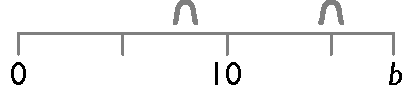
\includegraphics[width=.3\textwidth]{img/samplesetup}

% Assume that the pulsar's period is $4$, so unsheltered Tycho would take damage at times $4$, $8$, $12$, etc.
% If Tycho leaves from the starting position (where it's sheltered) at time $0$, it can reach the first shelter after $8$ seconds, incurring radiation damage $d$ at time $4$ (but none at time $8$ because it's sheltered then).
% Continuing without stopping, it reaches the home base at time $18$, incurring $d+d$ more units of radiation damage (at times $12$ and $16$, respectively).
% This way it incurs $d+d+d=3d$ units of radiation damage and $18$ units of environmental damage.
% If instead Tycho waits at the $2$nd shelter (at position $15$) for $1$ second, the pulse at time $16$ causes it no damage, and it reaches the home base at time $19$ with a total of $2d + 19$ units of damage.
% This is better for most values of $d$.
% The two situations are shown here:
Припустимо, що період випромінювання пульсара дорівнює $4$, тому якщо Tycho не заховується в укритті, він отримуватиме пошкодження у моменти часу $4$, $8$, $12$ тощо.
Якщо Tycho вирушає зі стартової позиції (де він прихований від радіації) у час $0$, то він може дістатися до першого укриття через $8$ секунд, отримавши випромінювання $d$ у час $4$ (але не отримуючи випромінювання в час $8$, оскільки тоді він захищений).
Продовжуючи рух без зупинки, він дістається до бази в позиції $b$ в час $18$, зазнавши ще $d+d$ одиниць радіаційної шкоди (у часи $12$ та $16$ відповідно).
Таким чином, він зазнає $d+d+d=3d$ одиниць радіаційної шкоди та $18$ одиниць шкоди від навколишнього середовища.
Якщо ж Tycho зупиниться на другому укритті (у позиції $15$) на $1$ секунду, то у цей час удар пульсара у час $16$ не завдасть йому шкоди, і він дістанеться до бази в позиції $b$ в час $19$ із загальним дискомфортом $2d + 19$ одиниць.
Це краще для більшості значень $d$.
Обидві ситуації показані тут:

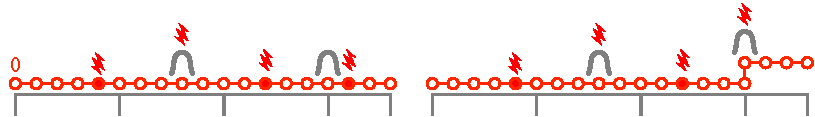
\includegraphics[width=.8\textwidth]{img/sample1_2.pdf}

% If the pulsar's period is $10$, Tycho can wait at the starting position for $2$~seconds and then just go home without stopping at any shelter.
% Thus it passes the $1$st shelter (at position~$8$) at just the right moment when the pulsar flares and arrives at the home base at time $20$, for a total of $20$ environmental damage and no radiation damage at all.
Якщо період пульсара дорівнює $10$, то Tycho може зачекати на початковій позиції протягом $2$~секунд, а потім просто повернутися додому, не зупиняючись в жодному укритті.
Таким чином, він проходить перше укриття (на позиції~$8$) саме в той момент, коли пульсар спалахує і прибуває до дому в час $20$, із загальним збитком від навколишнього середовища $20$ і жодної шкоди від радіації.


\includegraphics[width=.4\textwidth]{img/sample3.pdf}

% \section*{Input}
\section*{Вхідні дані}

% The first line consists of four integers $b$, $p$, $d$, and $n$, separated by single spaces:
% the location $b$ of the home base,
% the pulsar's flare period~$p$,
% the additional radiation damage~$d$ caused by each flare of the pulsar,
% the number~$n$ of the shelters.
% The following $n$~lines each contain an integer giving the shelter locations $a_1$, $\ldots$, $a_n$, with
$0<a_1<\cdots <a_n< b$. % constraint:shelterbounds, constraint:sortedshelters
Перший рядок містить чотири цілих числа $b$, $p$, $d$ і $n$, розділені одинарним пробілом:
розташування домашньої бази $b$,
період спалахів пульсара $p$,
додаткові радіаційні збитки~$d$, спричинені кожним спалахом пульсара,
кількість прихистків~$n$.
Наступні $n$~рядків містять ціле число, що вказує розташування прихистків $a_1$, $\ldots$, $a_n$, де
$0<a_1<\cdots <a_n< b$. % constraint:shelterbounds, constraint:sortedshelters

% \section*{Output}
\section*{Вихідні дані}

% Print a single integer: the minimum amount of damage Tycho must take to reach $b$.
Виведіть одне ціле число: мінімальну кількість пошкоджень, яку Tycho повинен зазнати, щоб досягти місця призначення $b$.

% \section*{Constraints and Scoring}
\section*{Обмеження та оцінювання}

% You can assume
Ви можете припустити, що
$1\leq p < b$ % constraint:pulsehappens
% and
та
$0\leq n < b$. % constraint:sheltersfit
% We always have
Ми завжди маємо:
$1\leq b\leq 10^{12}$, % constraint:b
$0\leq d \leq 10^6$, %constraint:d
% and
та
$0\leq n \leq 10^5$. % constraint:n

% Your solution will be tested on a set of test groups, each worth a number of points.
% Each test group contains a set of test cases.
% To get the points for a test group you need to solve all test cases in the test group.
% Your final score will be the maximum score of a single submission.
Ваше рішення буде перевірено на наборі тестових груп, кожна з яких має певну кількість балів.
Кожна група містить певну кількість тестових випадків.
Щоб отримати бали за групу тестів, потрібно вирішити всі тестові випадки в цій групі.
Ваш кінцевий бал буде максимальним балом за одне відправлення.

\medskip
\begin{tabular}{lll}
% Group & Points & Constraints \\\hline
Група & Бали & Обмеження \\\hline
%  $1$ & $8$  & $p\leq 10^6$ and Tycho does not need to wait \emph{after} leaving position~$0$.$^*$ \\ % constraint:nowait
  $1$ & $18$  & $p\leq 10^6$ та Tycho не повинен чекати \emph{після} виходу з позиції~$0$.$^*$ \\ % constraint:nowait
  $2$ & $15$  & $b\leq 1000$, $p\leq 100$, $n\leq 10$ \\
  $3$ & $7$  & $b\leq 1000$ \\
  $4$ & $15$ & $p\leq 10^6$, $n\leq 1000$\\
  $5$ & $20$ & $p\leq 100$\\
  $6$ & $15$ & $p\leq 10^6$\\
%  $7$ & $10$ & \emph{No additional constraints}
  $7$ & $10$ & \emph{Без додаткових обмежень}
\end{tabular}

\medskip
% \noindent $^*$ In test group~$1$, Tycho may still need to wait at position~$0$ \emph{before} it starts moving.
% For example, sample inputs $2$, $3$, and $4$ belong to test group~$1$.
\noindent $^*$ У групі тестів~$1$ Tycho може все ще потрыбно чекати в позиції~$0$ \emph{перед} початком руху.
Наприклад, вхідні дані для прикладів $2$, $3$, та $4$ належать до групи тестів~$1$.
